\documentclass[11pt]{cernrep}
\usepackage{graphicx,epsfig}
\bibliographystyle{lesHouches}
\begin{document}


\title{Sensitivity of current (and future?) LHC measurements to a new light scalar particle}

\author{
J. M. Butterworth$^1$, 
S. Fichet$^2$,
L. Finco$^6$,
S. Gascon-Shotkin$^6$,
D. Grellscheid$^{4}$, 
G. Moreau$^3$,
P. Richardson$^{4,5}$, 
D. Yallup$^1$,
S. Zhang$^{6,7}$ 
}
\institute{$^1$Department of Physics \& Astronomy, UCL, London, WC1E 6BT, UK 
\\$^2$ICTP-SAIFR \& IFT-UNESP, R. Dr. Bento Teobaldo Ferraz 271, S\~ao Paulo, Brazil
\\$^3$Laboratoire de Physique Th\'eorique, B\^at. 210, CNRS, Univ. Paris Sud, Universit\'e Paris-Saclay, F-91405 Orsay Cedex, France
\\$^4$IPPP, Department of Physics, Durham University, UK
\\$^5$Theory Department, CERN, Geneva, Switzerland
\\$^6$ Univ. Lyon, Universit\'e Claude Bernard Lyon 1, CNRS/IN2P3, UMR5822 IPNL,  F-69622 Villeurbanne, France
\\$^7$Institute of High Energy Physics/University of the Chinese Academy of Sciences, 19B Yuquan Road, Shijingshan District, Beijing, China 100049
}

\maketitle

\begin{abstract}
Additional scalar particles are a generic feature of many well-motivated extensions of Standard Model. 
Here we use a simplified model in which a light scalar particle couples to electroweak gauge bosons via dimension-5 operators. For the masses considered, decays to pairs of weak bosons are suppressed,
and the $\gamma\gamma$ mode dominates. We find that existing measurements from Run I of the LHC already exclude the model over a significant parameter range. 

\end{abstract}

\section{INTRODUCTION}

Additional light scalar particles are a common feature in extensions of the SM, for example appearing in composite 
Higgs scenarios, or as the radion in models with extra dimensions~\cite{Angelescu:2017jyj}. 
Consideration of precision electroweak measurements, collider searches and flavour physics
does not completely exclude the existence of light neutral CP-odd or CP-even scalar particles below the mass of the 
observed Higgs boson\cite{Cacciapaglia:2016tlr}. In this contribution we use a simplified  model 
to examine whether measurements from Run I at the LHC can give information about such possible particles.

\section{THE MODEL}

We use an effective theory (EFT) approach to describe a scalar with mass $M_\phi$ interacting with gauge bosons. The effective theory has $SU(2)\times U(1)_Y$ symmetry. This EFT gives a generic parametrization if $M_\phi\gg v$ \cite{Fichet:2015yia}, where $v$ is the electroweak scale.
 Whenever the scalar is light so that $M_\phi\gg v$ is not true, we make the extra assumption that the scalar has large tree-level $SU(2)\times U(1)_Y$ couplings, so that the loop-induced electroweak-breaking contributions are subleading. 
Under these conditions the interactions of a CP-even and CP-odd scalars with gauge bosons are respectively described by the following dimension-5 effective Lagrangians 
\begin{equation}
{\cal L}_{\rm eff}\supset\phi \left( \frac{1}{f_G}G^{\mu\nu\,a}G_{\mu\nu}^a+ \frac{1}{f_W}W^{\mu\nu\,I}W_{\mu\nu}^I
+\frac{1}{f_B}B^{\mu\nu}B_{\mu\nu}+\frac{1}{f_H}|D^\mu H|^2
\right)
\end{equation}
\begin{equation}
{\cal L}_{\rm eff}\supset\phi \left( \frac{1}{f_G}G^{\mu\nu\,a}\tilde G_{\mu\nu}^a+ \frac{1}{f_W}W^{\mu\nu\,I}\tilde W_{\mu\nu}^I
+\frac{1}{f_B}B^{\mu\nu}\tilde B_{\mu\nu}
\right)
\end{equation}
where $\tilde V^{\mu\nu}=\frac{1}{2}\epsilon^{\mu\nu\rho\sigma}V_{\rho \sigma}$.
The effective theory is valid as long as the $f$'s are larger than the energy going through the vertices. 
 Mixing with the SM Higgs is assumed to be small to ensure that the SM Higgs has SM-like  couplings compatible with  observations.

The CP-even scalar can for instance be identified as the radion mode present in warped extra-dimension models with bulk gauge fields. Interestingly, if EW brane kinetic terms are negligible in such models, one has $f_W=f_B$ \cite{Fichet:2013ola, Fichet:2013gsa}, which implies that the $\phi F^{\mu\nu}Z_{\mu\nu}$ coupling vanishes, a property which can be used for model discrimination \cite{Baldenegro:2017aen}. 
The CP-odd scalar is typically a pseudo Nambu Goldstone boson from an approximate global symmetry, just like those appearing in composite Higgs models. The couplings to gauge fields are induced by the many fermion resonances populating the TeV scale (see e.g \cite{Belyaev:2016ftv} or also \cite{Fichet:2016xvs}). 



In the following, as a first exercise, we assume a common scale $\Lambda$ for all couplings,
\begin{equation}
f_G \sim f_B\sim f_W\sim f_H\sim \Lambda \,,
\end{equation}
and similarly for the CP-odd case. 


\section{SENSITIVITY OF EXISTING MEASUREMENTS}

\subsection{Herwig Implementation}

The new processes defined by the model described above are exported as UFO file~\cite{Degrande:2011ua} which is 
read by Herwig~7.2.1~\cite{Bellm:2015jjp,Bahr:2008pv}. This requires the four-boson vertices, 
which were added to the Herwig UFO interface as part of this work 
and are now available in this subsequently released version. The five-boson vertices implied by the model 
are not yet implemented
but are assumed not to have a major impact. 
This assumption is supported by a cross-check using MadGraph5\_aMC@NLO\_v2\_5\_5~\cite{MadGraph} for a selection of the parameter points considered. MadGraph5\_aMC@NLO
includes the full set of vertices, as well as some higher-order QCD contributions; the cross sections predicted by MadGraph5\_aMC@NLO are 
generally higher than the Herwig values, but are consistent with a factor of two. Thus any limits derived using Herwig are likely to
be somewhat conservative.

The scale which suppresses couplings to the 
Higgs and weak bosons is varied across the range $1 < \Lambda < 10$~TeV; all other BSM coupling are heavily 
suppressed ($\Lambda = 1000$~TeV). All
allowed $\phi$-production processes are generated inclusively.

\subsection{Rivet and Contur}

Generated Herwig events are passed to the Rivet library of analysis routines~\cite{Buckley:2010ar}. This contains 
a signficant number of published ATLAS and CMS analyses. Measurements which have been corrected for detector effects
to a particle-level fiducial phase space are rather model-independent. Rivet allows the particle-level analysis as performed
by the experiments to be applied to the BSM events generated by Herwig. Since the measurements considered 
have all been compared to precision SM calculations and shown to agree, there is limited room for additional BSM contributions.
The Contur comparison package~\cite{Butterworth:2016sqg} quantifies the level of contribution which could still be 
consistent with the data. Currently this is done on the assumption that the data are identical to the SM; a more
complete approach would be to use the SM predictions and their uncertainties directly; such a capability is a planned
future development of Contur, but the present implementation is enough to give a reasonable indication of the 
sensitivity of the data to BSM models.

\subsection{Measurements}

All available ATLAS and CMS Rivet analyses are used to study the data. However, since the branching ratio 
$\phi \rightarrow \gamma\gamma$ is $\approx 1$, the measurements of interest are those involving
isolated photons, or pairs of photons, in the final state. These have been measured 
inclusively~\cite{Aad:2012tba,Aad:2013zba,Aad:2016xcr}, and in 
association with jets~\cite{Chatrchyan:2013mwa,Aad:2013gaa,ATLAS:2012ar}, $W$ or $Z$ bosons\cite{Aad:2013izg,Aad:2016sau} (i.e. leptons and/or missing energy). 

The Higgs fiducial diphoton measurements~\cite{Aad:2014lwa} are also of interest. These were studied and in principle 
have some sensitivity -- events generated by the models considered do contribute to the fiducial region. However, since 
the value of $M_\phi$ considered here lie below the SM Higgs mass, the events which will enter the fiducial phase space
of the Higgs measurement will arise from combinatorial backgrounds of pairs of photons, and thus will not exhibit a 
peak at the Higgs mass. Because of this, they are likely to removed as part of the background fitting and subtraction 
process in that analysis. We therefore do not include the Higgs cross sections when calculating the exclusion limits.

\subsection{Results}

For the CP-even scalar, the cross section in 8 TeV $pp$ collisions calculated by Herwig ranges from 
110~pb for $\Lambda = 1$~TeV to 1.3~pb for $\Lambda = 10$~TeV for $M_\phi = 10$~GeV,
and from 
8.2~pb for $\Lambda = 1$~TeV to 0.12~pb for $\Lambda = 10$~TeV for $M_\phi = 90$~GeV.
For the CP-odd scalar, the cross section in 8 TeV $pp$ collisions calculated by Herwig ranges from 
15~pb for $\Lambda = 1$~TeV to 0.26~pb for $\Lambda = 10$~TeV for $M_\phi = 10$~GeV,
and from 
4.3~pb for $\Lambda = 1$~TeV to 0.077~pb for $\Lambda = 10$~TeV for $M_\phi = 90$~GeV. In all cases, the 
associated production of $\phi$ with a $Z$ or $W$ boson makes the biggest contribution to the cross section, 
although the $\phi + \gamma$ process is significant (10-20\%), and the $\phi + g$ process contributes up to
20\% (40\%) for the highest scale and mass values considered for the CP even (odd) scalar.

At low $M_\phi$ and low-ish $\Lambda$, one of the most sensitive measurements is the $\gamma+E_T^{\rm miss}$ measurement 
from \cite{Aad:2013izg}. The differential cross section as a function of the transverse momentum of the photon 
is shown in Fig.~\ref{fig:cpo_lowlow}, and alone is enough to excludes the model at the 97\% cl.
The inclusive photon measurements are also sensitive, with the 7~TeV diphoton measurement extending to
the lowest mass and $p_T$ values, and the 8~TeV measurement (shown) playing a role once $M_\phi \geq 20$ GeV.

\begin{figure}
\begin{center}
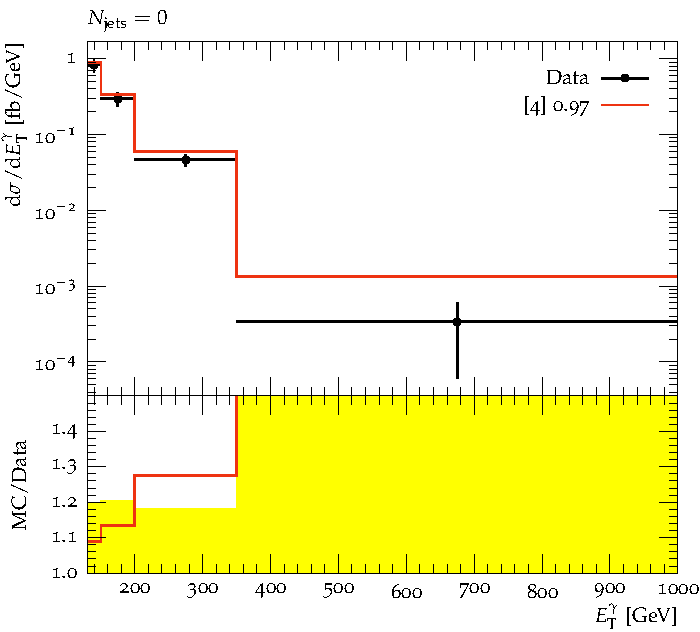
\includegraphics[width=0.49\textwidth]{ATLAS_2016_I1448301_NU_d08-x01-y01-10-3500.pdf}
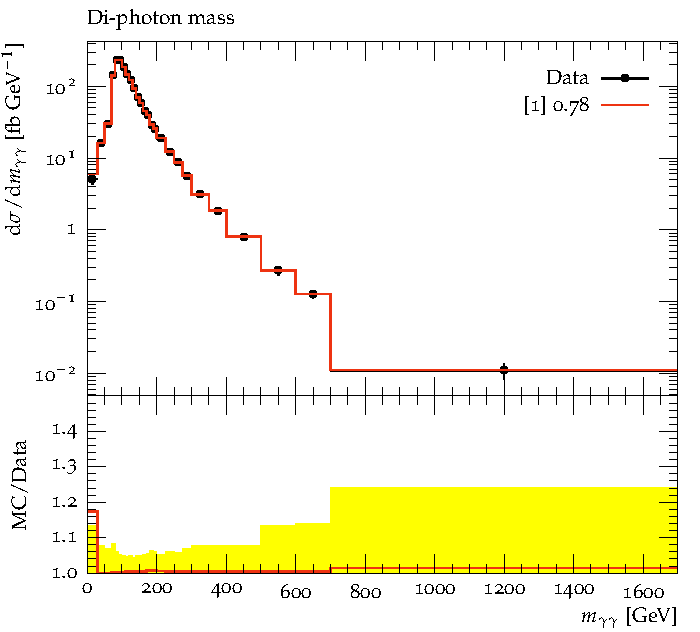
\includegraphics[width=0.49\textwidth]{ATLAS_2017_I1591327_d02-x01-y01-20-3500.pdf}
    \caption{Projection of the contribution of the CP-odd model, (left) for $M_{\phi} = 10$~GeV and $\Lambda = 3500$~TeV, on to the 
8 TeV ATLAS $\gamma+E_T^{\rm miss}$ differential $E_T^\gamma$ cross-section measurement  and (right) on the 
diphoton mass measurement, now with $M_{\phi} = 20$~GeV -- which brings the mass peak from the $\phi$ within
the range of the measurement.
Black points indicate the data, the red upper histogram is the data+BSM. The lower sections of the plots show the ratio of 
(data+BSM)/data, with the yellow band indicating the uncertainty in the measurement. 
The numbers in the legend show the bin number of the most powerful bin, and the exclusion from that bin expressed as a 
probability.}
\label{fig:cpo_lowlow}
\end{center}
\end{figure}

As mentioned in the previous section, events from the model can contribute to the Higgs fiducial two-photon cross section,
and this is seen in the Rivet routine. The major contribution occurs for relatively low $M_\phi$, presumably due to 
$pp \rightarrow \gamma \phi + X \rightarrow \gamma \gamma \gamma + X$ processes in which one pair 
of photons has a mass close to 125~GeV. An example, for $M_\phi = 20$~GeV, $\Lambda = 3.5$~TeV, is shown in Fig.~\ref{fig:higgs_and_cp}.
The event contribute mainly at low values of $p_T$ for the photon pair. As discussed, this analysis is not used in deriving
the final sensitivity, and is shown only for illustration. {\bf TODO check this. Looks like it is used.}

\begin{figure}
\begin{center}
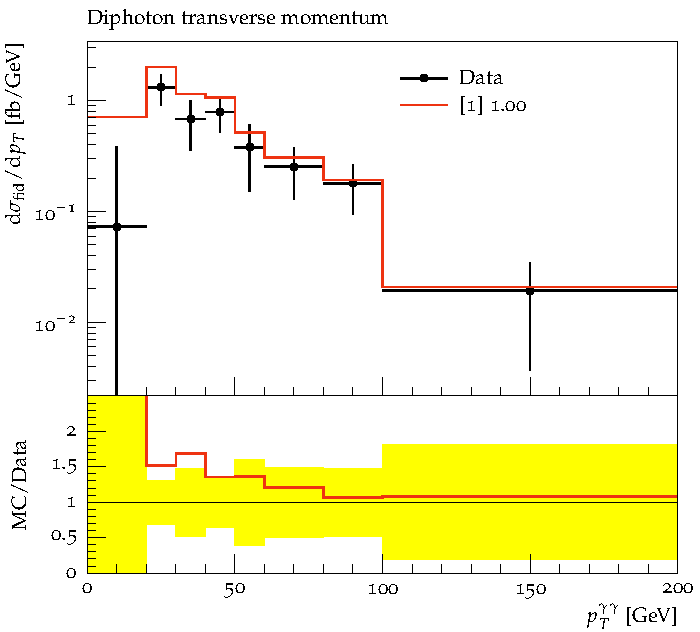
\includegraphics[width=0.49\textwidth]{ATLAS_2014_I1306615_d01-x01-y01-20_3500.pdf}
%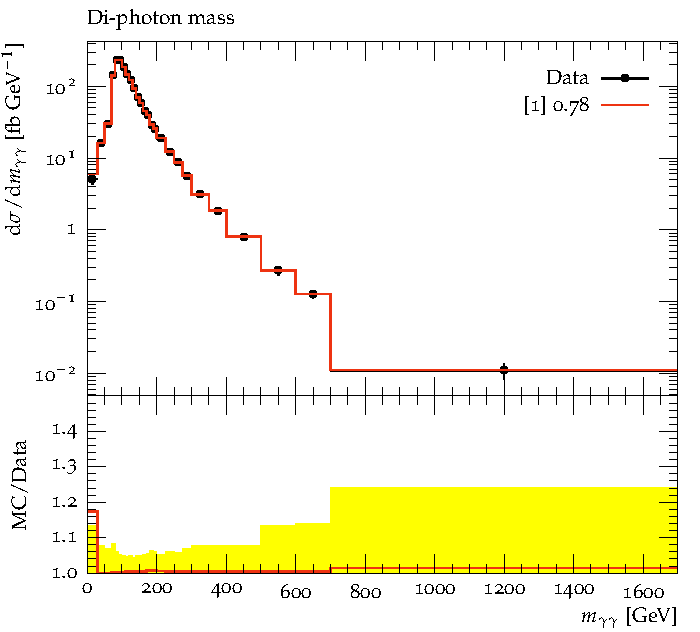
\includegraphics[width=0.49\textwidth]{ATLAS_2017_I1591327_d02-x01-y01-20-3500.pdf}
    \caption{Projection of the contribution of the CP-odd model, for $M_{\phi} = 20$~GeV and $\Lambda = 3500$~TeV, on to the 
8 TeV ATLAS $H \rightarrow \gamma\gamma$ differential $p_T^{\gamma\gamma}$ cross-section measurement.
Legend as Fig.\protect\ref{fig:cpo_lowlow}}
\label{fig:higgs_and_cpo}
\end{center}
\end{figure}

The CP-even model contributes to the same final states, but with a larger cross section for a given coupling. The distributions
for the this model with the same parameter settings as Fig.~\ref{fig:cpo_lowlow} are shown in Fig.\ref{fig:cpe_lowlow}

\begin{figure}
\begin{center}
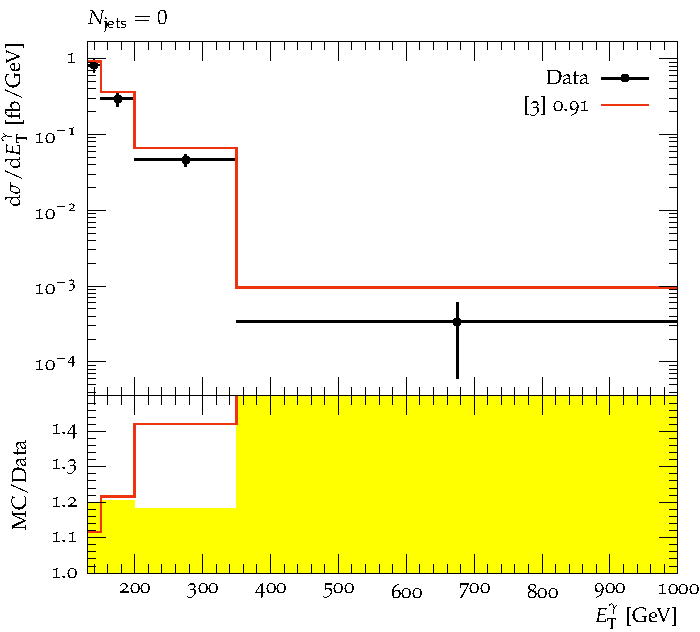
\includegraphics[width=0.49\textwidth]{ATLAS_2016_I1448301_NU_d08-x01-y01-10-3500e.pdf}
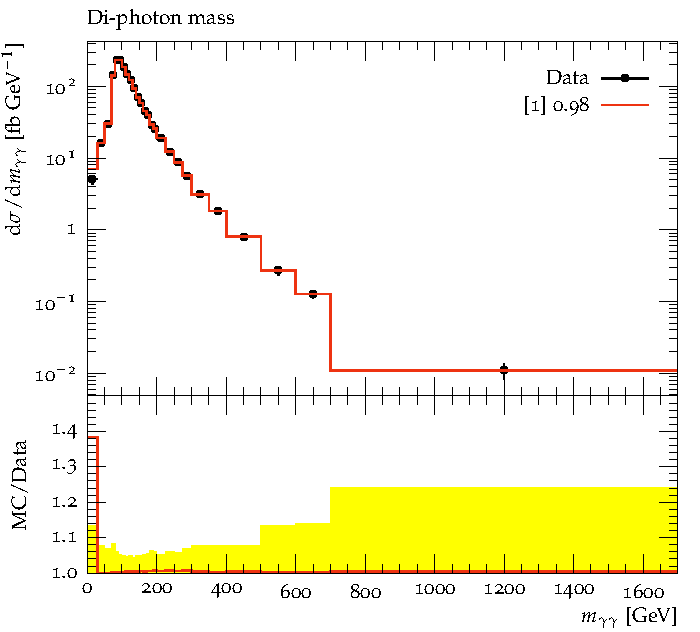
\includegraphics[width=0.49\textwidth]{ATLAS_2017_I1591327_d02-x01-y01-20-3500e.pdf}
    \caption{Projection of the contribution of the CP-even model, for $M_{\phi} = 10$~GeV and $\Lambda = 3500$~TeV, on to the 
8 TeV ATLAS $\gamma+E_T^{\rm miss}$ differential $E_T^\gamma$ cross-section measurement (left) and (right) the 
diphoton mass measurement playing a role now with $M_{\phi} = 20$~GeV, which brings the mass peak from the $\phi$ within
the range of the measurement.
Legend as Fig.\protect\ref{fig:cpo_lowlow}}
\label{fig:cpe_lowlow}
\end{center}
\end{figure}

The sensitivity of the combined 7 and 8 TeV data to the CP-odd scalar model is illustrated in Fig.~\ref{fig:cpomaps}.
Dependent on $M_\phi$, the $\Lambda$ values up to 4.5 to 8.5~TeV are excluded, under the assumptions of our procedure. 
Similar sensitivity plots for the CP-even model are shown in Fig.~\ref{fig:cpemaps}. comment on the range.
Precision 13~TeV data can be expected to extend the reach still further; possible dedicated analyses which might extend the
sensitivity still further are discussed in the following section.

\begin{figure}
\begin{center}
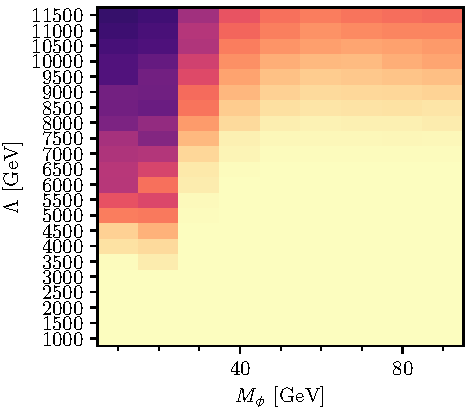
\includegraphics[width=0.49\textwidth]{cpo-wz-map.pdf}
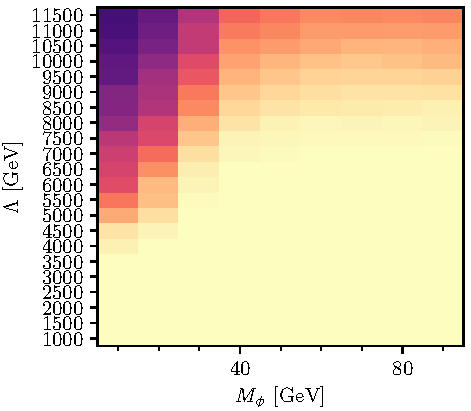
\includegraphics[width=0.49\textwidth]{cpo-gg-map.pdf}
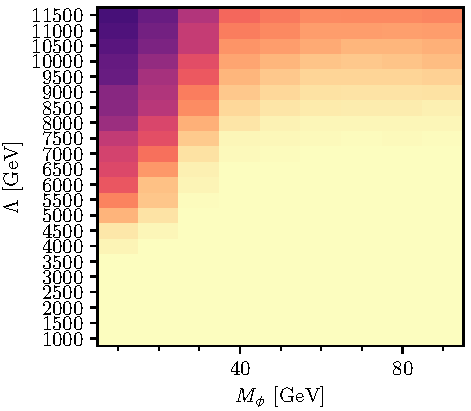
\includegraphics[width=0.49\textwidth]{cpo-map.pdf}
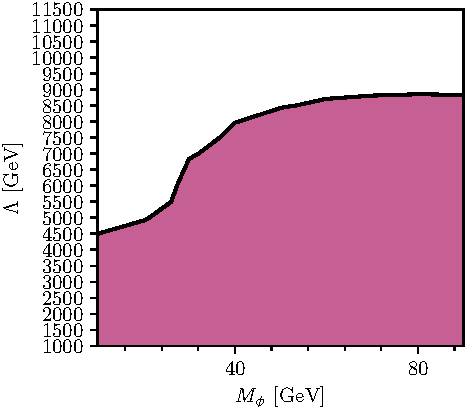
\includegraphics[width=0.49\textwidth]{cpo-contour.pdf}\\
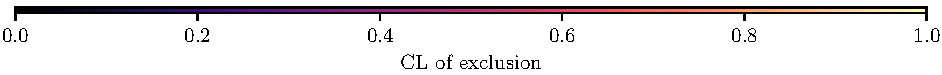
\includegraphics[width=0.99\textwidth]{colorbarkey.pdf}
    \caption{CP-odd scalar model: Top left, exclusion heatmap (with the key below the figure) for 
7 \& 8 TeV diboson measurements (i.e. final states consistent with $WW, ZZ, W+\gamma(\gamma), Z+\gamma(\gamma)$) 
from ATLAS and CMS. Top right, exclusion heatmap for 7 \& 8 TeV photon and diphoton measurements, lower left combined 
exclusion heatmap, bottom right, combined exclusion contour at 95\% c.l.}
\label{fig:cpomaps}
\end{center}
\end{figure}

\begin{figure}
\begin{center}
%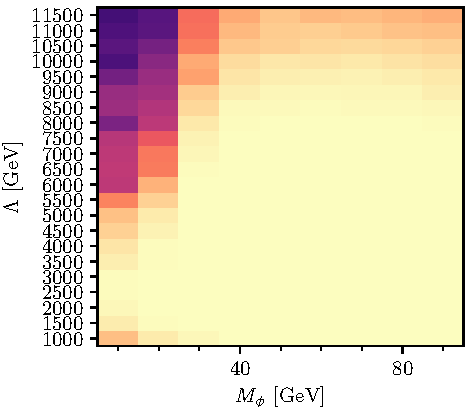
\includegraphics[width=0.49\textwidth]{cpe-wz-map.pdf}
%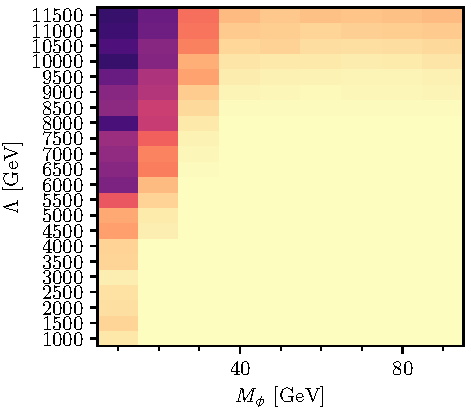
\includegraphics[width=0.49\textwidth]{cpe-gg-map.pdf}
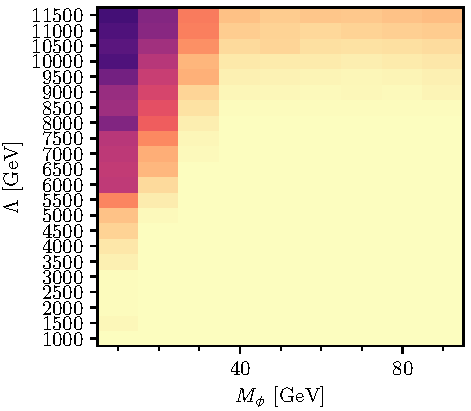
\includegraphics[width=0.49\textwidth]{cpe-map.pdf}
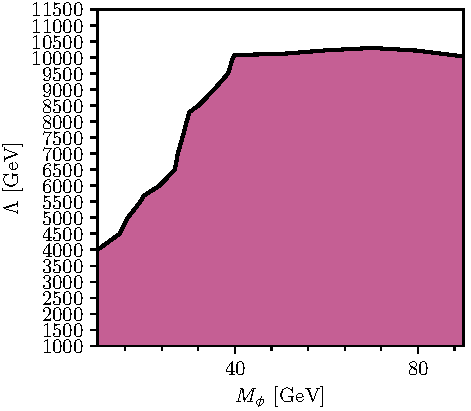
\includegraphics[width=0.49\textwidth]{cpe-contour.pdf}\\
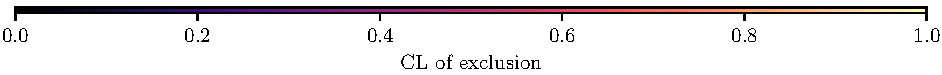
\includegraphics[width=0.99\textwidth]{colorbarkey.pdf}
    \caption{As the lower row of Fig.\protect\ref{fig:cpomaps}, but for the CP-even scalar model.}
\label{fig:cpemaps}
\end{center}
\end{figure}

%\section{FUTURE PROSPECTS}

%Or checks of the above using MadGraph?
%Susan, Linda, Sijing?

\section*{CONCLUSIONS}
The generic light scalar models considered here imply significant contributions to differential cross sections involving 
weak bosons and/or isolated photons which have already been measured at the LHC and shown to be consistent with the Standard Model. 
While a rigorous exclusion would require a treatment of the theory uncertainties on the SM photon cross sections, these models
can be considered highly disfavoured for scales below about 4~TeV for $M_\phi = 10$~GeV and up to about 8.5~TeV for 
$M_\phi = 90$~GeV.


\section*{ACKNOWLEDGEMENTS}
We thank the organizers and conveners of the Les Houches workshop, ``Physics
at TeV Colliders'', for a stimulating meeting.
This work has received funding from STFC (UK), and the European Union's Horizon 2020 research and innovation programme 
as part of the Marie Sklodowska-Curie Innovative Training Network MCnetITN3 (grant agreement no. 722104).

\bibliography{lightscalar}

\end{document}
